% =============================================================
%  lecture.tex
%  Master file for IPhO Training Lecture Notes (textbook build).
%
%  To compile:    pdflatex lecture.tex
%
%  Each topic lives in its own file under this directory and is
%  brought in via \input below.  Add new chapters by:
%      1. creating <topic>.tex that begins with `\chapter{...}`
%      2. listing it in the "Main matter" block below
% =============================================================

\documentclass[11pt,a4paper,openany]{book}

% ---------- core math + symbols ----------
\usepackage{amsmath,amssymb,amsthm,mathtools}
\usepackage{bm}

% ---------- layout ----------
\usepackage[a4paper,margin=1in]{geometry}
\usepackage{parskip}        % blank line between paragraphs, no first-line indent
\usepackage{enumitem}
\usepackage{microtype}
\usepackage{framed}

% ---------- fonts ----------
\usepackage{fontspec}
\usepackage{unicode-math}

% ---------- graphics, color, links ----------
\usepackage{wrapfig}
\usepackage{graphicx}
\usepackage{subcaption}
\usepackage{xcolor}
\usepackage[hidelinks,
            colorlinks=true,
            linkcolor=blue!60!black,
            urlcolor=blue!60!black,
            citecolor=blue!60!black]{hyperref}

% ---------- nicer chapter / section headings ----------
\usepackage[explicit]{titlesec}
\titleformat{\chapter}[display]
    {\normalfont\Huge\bfseries}
    {\filright\Large\chaptertitlename\ \thechapter}
    {1ex}
    {\titlerule\vspace{1ex}\filright #1}
\titlespacing*{\chapter}{0pt}{-30pt}{30pt}

% ---------- theorem-like environments ----------
\theoremstyle{plain}
\newtheorem{theorem}{Theorem}[chapter]
\newtheorem{proposition}[theorem]{Proposition}
\newtheorem{corollary}[theorem]{Corollary}
\newtheorem{lemma}[theorem]{Lemma}

\theoremstyle{definition}
\newtheorem{definition}[theorem]{Definition}
\newtheorem{example}[theorem]{Example}

\theoremstyle{remark}
\newtheorem{remark}[theorem]{Remark}
\newtheorem*{note}{Note}

% ---------- shared math shorthand ----------
% (Sub-files can \providecommand the same names; first definition wins.)
\newcommand{\dd}{\mathrm{d}}
\newcommand{\dbar}{\mathop{\overline{\mathrm{d}}}}    % inexact differential
\newcommand{\pd}[2]{\dfrac{\partial #1}{\partial #2}}
\newcommand{\pa}[2]{\left(\dfrac{\partial #1}{\partial #2}\right)}
\newcommand{\avg}[1]{\left\langle #1 \right\rangle}
\newcommand{\tr}{\operatorname{tr}}
\newcommand{\zh}[1]{{\fontspec{AR PL KaitiM Big5} #1}}
\newcommand{\sgn}{\operatorname{sgn}}
\newcommand{\E}{\bar{E}}
\newcommand{\N}{\bar{N}}

% ---------- metadata ----------
\title{
    \vspace{2cm}
    {\Huge\bfseries Selected Topics in Physics}\\[0.5em]
    {\Large Lecture Notes for IPhO Training}
    \vspace{1cm}
}
\author{Hung-Wei}
\date{\today}

\begin{document}

\frontmatter
\maketitle

\tableofcontents

% =============================================================
\mainmatter
% =============================================================

% ---- Main matter: one \input per chapter ----
% =============================================================
%  classical_thermodynamics.tex
%  Lecture notes on classical thermodynamics for IPhO training.
%  Intended to be \input from lecture.tex (no \documentclass /
%  \begin{document} here).  The parent file should provide:
%      \usepackage{amsmath,amssymb,amsthm,mathtools}
%      \usepackage{bm}
%      \usepackage{enumitem}
%      (and any theorem-environment definitions one wants)
% =============================================================

% --- shorthand commands used below --------------------------------------
\providecommand{\dd}{\mathrm{d}}
\providecommand{\dbar}{\mathchar'26\mkern-12mu\mathrm{d}}  % inexact differential
\providecommand{\pd}[2]{\dfrac{\partial #1}{\partial #2}}
\providecommand{\pa}[2]{\left(\dfrac{\partial #1}{\partial #2}\right)}

% =============================================================
\chapter{Classical Thermodynamics}
% =============================================================

\noindent\textit{Reference: A.~H.~Carter, \emph{Classical and Statistical Thermodynamics}, Chapters~1--6.}

%==============================================================
\section{Zeroth and First Laws}
%==============================================================

\subsection{Some Basic Definitions}

\paragraph{Open, closed and isolated systems.}
\begin{itemize}
    \item An \emph{open system} can exchange both energy and matter with its surroundings.
    \item A \emph{closed system} can exchange energy but not matter (the walls are impermeable, but heat and work can still flow).
    \item An \emph{isolated system} can exchange neither: no heat, no work, no particles.
\end{itemize}

\paragraph{Properties/ State functions.}
A (thermodynamic) \emph{property}, or a \emph{state function}, is a quantity associated to a system's state. It 
has nothing to do with processes or paths; it is a function of the current macroscopic state only.

\textcolor{blue}{Question: For a system with fixed number of particles, how many independent state functions are needed to specify the state of the system?}

\paragraph{Intensive vs.\ extensive properties.}
A property is \emph{extensive} if doubling the size of the system doubles its value, and \emph{intensive} if it remains unchanged. Examples:
\begin{center}
\begin{tabular}{ll}
    \textbf{Extensive:} & $V$ (volume), $N$ (number of particles), $U$ (internal energy), $S$ (entropy)\\
    \textbf{Intensive:} & $T$ (temperature), $P$ (pressure), $\rho$ (density), $\mu$ (chemical potential)
\end{tabular}
\end{center}

\paragraph{Non-State functions.}
By contrast, heat $Q$ and work $W$ are \emph{not} state functions --- their definitions 
depend on the process, usually through a integral along that process. 

\paragraph{Reversible and quasi-static processes.}
\begin{itemize}
    \item A process is \emph{quasi-static} if it is carried out slowly enough that the system passes through a continuous sequence of equilibrium states. Each intermediate state can be plotted as a point in (e.g.) the $P$--$V$ plane.
    \item A process is \emph{reversible} if it is quasi-static \emph{and} produces no net dissipation, so it can be retraced in the opposite direction without leaving any change in the surroundings.
\end{itemize}
All reversible processes are quasi-static, but not vice versa. 
%--------------------------------------------------------------
\subsection{Basic Axioms}

The ``laws'' of classical thermodynamics are \emph{axioms}; 
they are not derived from anything more fundamental, thus cannot be proved.

\paragraph{Zeroth Law.}
\begin{quote}
\textit{If body $A$ is in thermal equilibrium with body $B$, and body $B$ is in thermal equilibrium with body $C$, then $A$ is also in thermal equilibrium with $C$.}
\end{quote}

\paragraph{Why this matters.}
The zeroth law allows us to define a unique state function, temperature $T$, which 
is a function of $P$ and $V$. 

See the link \url{https://chatgpt.com/share/6a2a1a67-af90-8324-9088-46a92193deea} for more details.

Once $T$ exists, a simple system in mechanical equilibrium has the macroscopic variables $(P,V,T)$. These are not independent: there is one constraint (the \emph{equation of state}), so the system has two degrees of freedom. For an ideal gas the equation of state is the familiar
\[
    PV = nRT.
\]
For real substances the equation of state is more complicated (van der Waals, virial expansion, etc.) but the count of variables and constraints is the same.

%==============================================================
\section{Work, Heat, and the First Law}
%==============================================================

\subsection{The First Law}

\begin{quote}
\textbf{Axiom (First Law).} \textit{Heat is a form of energy, and energy is conserved.}
\end{quote}
In differential form,
\[
    \boxed{\,\dd U = \dbar Q + \dbar W\,}.
\]
Here $U$ is the \emph{internal energy} of the system, $\dbar Q$ is the heat absorbed by the system, and $\dbar W$ is the work done \emph{on} the system. 
\paragraph{Remarks.}
\begin{itemize}
    \item The First Law states that even though $Q$ and $W$ are path dependent, their sum $\dd U$ is an exact differential --- that is, $U$ is a state function. (Joule's paddle-wheel experiment)
    \item The First Law applies to \emph{irreversible} processes as well. However, in an irreversible process $\dbar W \neq -P\,\dd V$ in general: one must use the \emph{external} pressure that is doing the squeezing, not the (possibly undefined) internal pressure.
    \item Sign conventions differ between textbooks. We adopt ``work done \emph{on} the system'', so reversible compression gives $\dbar W = -P\,\dd V > 0$ for $\dd V < 0$. 
\end{itemize}

%--------------------------------------------------------------
\subsection{Four Processes and Heat Capacities}

\paragraph{Constants-volume processes.}
If the volume is held fixed and we ignore any exotic forms of work, $\dbar W = 0$ so $\dd U = \dbar Q$. Therefore
\[
    \pa{U}{T}_{V} = \pa{Q}{T}_{V} \equiv C_V.
\]
$C_V$ is a state-function derivative, while $(\dbar Q/\dd T)_V$ is the operationally measurable quantity (the heat needed per unit temperature rise at fixed $V$).

\paragraph{Enthalpy and constant-pressure processes.}
Define the \emph{enthalpy}
\[
    H \equiv U + PV.
\]
$H$ is also a state function (it is built from state functions). Its differential is
\[
    \dd H = \dd U + P\,\dd V + V\,\dd P = \dbar Q + V\,\dd P,
\]
where in the last step we used $\dd U = \dbar Q - P\,\dd V$ (i.e.\ reversible $P\,V$-work only). At constant pressure $\dd P = 0$ and hence
\[
    \pa{H}{T}_{P} = \pa{Q}{T}_{P} \equiv C_P.
\]

\paragraph{Isothermal processes and Adiabatic processes.}
We don't have much to say here yet, without the assumption of and ideal gas. We'll talk about them more in the next section. 

%--------------------------------------------------------------

\subsection{Ideal Gas}
The properties introduced in this section \textbf{only apply to ideal gas}. 
\paragraph{A. Ideal gas in isothermal and adiabatic processes.}
\begin{theorem}
    For ideal gases,
    \begin{itemize}
        \item \textbf{Isothermal} ($\dd T = 0$, ideal gas): $\dd U = 0$, so $\dbar Q = -\dbar W = nRT\,\dd V/V$. Integrating, $W_{\text{on}} = -nRT\ln(V_f/V_i)$.
        \item \textbf{Adiabatic} ($\dbar Q = 0$): the standard derivation gives $PV^\gamma = \mathrm{const}$ and $TV^{\gamma-1} = \mathrm{const}$, where $\gamma = C_P/C_V$.
    \end{itemize}   
\end{theorem}
\begin{proof}
    I bet you've seen this before. Skipped.
\end{proof}

\paragraph{B. U and H only depends on energy.}
\begin{theorem}
    For ideal gases, 
    \[
        \left.\pa{U}{V}\right|_T = 0, \qquad \left.\pa{H}{P}\right|_T = 0.
    \]
\end{theorem}
\begin{proof}
    Found through an experiment. See section \ref{sec:JT_coeff}. 
\end{proof}

\paragraph{C. Mayer's Relation.} 
\begin{theorem}
    $C_P - C_V = nR$ for an ideal gas. 
\end{theorem}

\begin{proof}
    Take $T$ and $V$ as independent variables. From $U=U(T,V)$,
\[
    \dd U = \pa{U}{T}_V \dd T + \pa{U}{V}_T \dd V = C_V\,\dd T + \pa{U}{V}_T \dd V.
\]
Combining with the First Law $\dd U = \dbar Q - P\,\dd V$ (reversible work) gives
\[
    \dbar Q = C_V\,\dd T + \left[P + \pa{U}{V}_T\right]\dd V.
\]
For an ideal gas, the Gay-Lussac/Joule expansion experiment shows $\pa{U}{V}_T = 0$ (more on this in a moment), so
\[
    \dbar Q = C_V\,\dd T + P\,\dd V.
\]
Now switch to $T$ and $P$ as the independent variables using $PV=nRT$, so $P\,\dd V + V\,\dd P = nR\,\dd T$, i.e.\ $P\,\dd V = nR\,\dd T - V\,\dd P$. Substituting,
\[
    \dbar Q = (C_V + nR)\,\dd T - V\,\dd P.
\]
Reading off the coefficient at constant $P$ ($\dd P = 0$),
\[
    \boxed{\,C_P = C_V + nR\,}.
\]
\end{proof}
\subsection{Exercise.}
\zh{
\textbf{2020 複選P1.}

(A) 奧圖（Otto）引擎為內燃機常見的型態。其運轉步驟如圖1所示：

$1 \to 2$ 與 $3 \to 4$ 為絕熱過程，$2 \to 3$ 與 $4 \to 1$ 為等體積過程。試求奧圖引擎之效率 $e_O$。

(B) 阿特金森（Atkinson）引擎為由奧圖引擎改良而來，近年來越來越常見於私家車輛上。

其標準運轉步驟如圖2所示：
$1 \to 2$ 與 $3 \to 4$ 為絕熱過程，$2 \to 3$ 為等體積過程，而 $4 \to 1$ 近似等壓過程。

阿特金森引擎基本精神為，與奧圖引擎相較，降低壓縮比
$r_C = \frac{V_2}{V_1}$ 來減少燃燒油氣量，

但仍具有相同的對外作功膨脹比
$r_E = \frac{V_4}{V_3}$。試求阿特金森引擎之效率 $e_A$。

(C) 比較 $r_C$ 相同（燃燒室容量／燃料相同）的奧圖引擎與阿特金森引擎，

試定量比較兩個引擎的效率，何者效率較高？
}

\begin{center}
    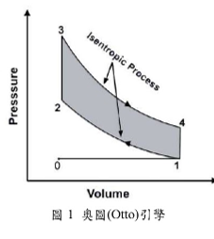
\includegraphics{../Figure/Otto_engine.png}
    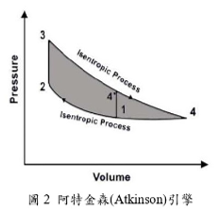
\includegraphics{../Figure/atkinson_engine.png}
\end{center}

\paragraph{Solution.}
\textbf{(A)}
\begin{align*}
W_{\text{total}} &= W_{3 \to 4} + W_{1 \to 2} \quad \text{Since } 1 \to 2 \text{ and } 3 \to 4 \text{ are \zh{絕熱},} \\
&= - (\Delta U_{3 \to 4} + \Delta U_{1 \to 2}) \\
&= - nkR (T_4 - T_3 + T_2 - T_1).
\end{align*}

\begin{align*}
Q_{\text{abs}} &= Q_{2 \to 3} \quad \text{since \zh{等體積},} \\
&= \Delta U_{2 \to 3} = n k R (T_3 - T_2).
\end{align*}

\begin{align*}
\Rightarrow e_O &= - \frac{T_4 - T_3 + T_2 - T_1}{T_3 - T_2} = 1 - \frac{T_4 - T_1}{T_3 - T_2} \\
&= 1 - \left( \frac{V_2}{V_1} \right)^{\gamma - 1}.
\end{align*}

\vspace{1em}
\textbf{(B)}
\begin{align*}
Q_{\text{abs}} &= k R (T_3 - T_2). \\
W_{\text{total}} &= W_{1 \to 2} + W_{3 \to 4} + W_{4 \to 1} \\
&= - kR (T_4 - T_3 + T_2 - T_1) + P_1 (V_1 - V_4).
\end{align*}

\begin{align*}
e_A &= \left[ 1 - \frac{T_4 - T_1}{T_3 - T_2} \right] + \frac{P_1(V_1 - V_4)}{n k R (T_3 - T_2)} \\
&= 1 - \frac{P_1 V_4 - P_1 V_1}{V_L (P_3 - P_2)} + \frac{1}{k} \cdot \frac{P_1 V_4 - P_1 V_1}{V_L (P_3 - P_2)} \\
&= 1 - \left( 1 + \frac{1}{k} \right) \cdot \frac{P_1 V_4 - P_1 V_1}{V_L (P_3 - P_2)} \\
&= 1 - \gamma \cdot \frac{V_4 - V_1}{V_L \left[ \left( \frac{V_4}{V_L} \right)^\gamma - \left( \frac{V_1}{V_L} \right)^\gamma \right]} \\
&= 1 - \gamma \frac{r_E - r_C^{-1}}{r_E^\gamma - r_C^{-\gamma}} = 1 - \gamma r_C^{\gamma - 1} \cdot \frac{r_C r_E - 1}{(r_C r_E)^\gamma - 1}.
\end{align*}

\vspace{1em}
\textbf{(C)}
\begin{align*}
\Rightarrow e_O &= 1 - r_C^{\gamma - 1} \\
e_A &= 1 - r_C^{\gamma - 1} \gamma \frac{x - 1}{x^\gamma - 1}, \quad \text{where } x = r_C r_E = \frac{V_4}{V_1} \\
e_A - e_O &= r_C^{\gamma - 1} \left( 1 - \gamma \frac{x - 1}{x^\gamma - 1} \right) = r_C^{\gamma - 1} \frac{(x^\gamma - 1) - \gamma(x - 1)}{x^\gamma - 1}.
\end{align*}

If $x > 1$, $x^\gamma - 1 > 0$. If $0 < x < 1$ and $\gamma > 1$, $x^\gamma - 1 < 0$.

Let $f(x) = (x^\gamma - 1) - \gamma(x - 1)$. $f(1) = 0$, $f(0) = \gamma - 1$.
\begin{align*}
f'(x) &= \gamma(x^{\gamma - 1} - 1) < 0 \quad \forall \ 0 < x < 1 \\
f'(x) &> 0 \quad \forall \ x > 1
\end{align*}
\begin{align*}
\Rightarrow \frac{x^\gamma - 1 - \gamma(x - 1)}{x^\gamma - 1} &< 0 \quad \forall \ 0 < x < 1, \\
&> 0 \quad \forall \ x > 1.
\end{align*}
%==============================================================
\section{The Second Law}
%==============================================================

\subsection{Heat Engines}

\begin{wrapfigure}{r}[1.5cm]{0.4\textwidth}
  \centering
  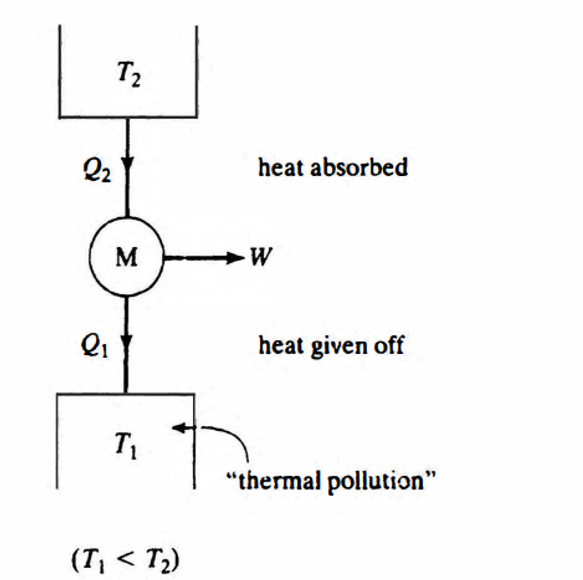
\includegraphics[width=0.4\textwidth]{../Figure/Heat_engine.png}
\end{wrapfigure}

A \emph{heat engine} is a cyclic device that absorbs heat $Q_2$ from a hot reservoir at $T_2$, releases heat $Q_1$ to a cold reservoir at $T_1<T_2$, and delivers net work $W = Q_2 - Q_1$. Its efficiency is
\[
    e \equiv \frac{W}{Q_2} = 1 - \frac{Q_1}{Q_2}.
\]
Universal experience tells us that some $Q_1>0$ is always wasted to the cold reservoir; you can never have $e=1$. The Second Law is the formalisation of this fact.

%--------------------------------------------------------------
\subsection{Axiomatic Statements}

\paragraph{Clausius statement.} \textit{No process is possible whose sole effect is the transfer of heat from a colder to a hotter body.}

\paragraph{Kelvin--Planck statement.} \textit{No heat engine can have efficiency $100\%$.} Equivalently, no cyclic device can convert heat entirely into work with no other effect.

The two statements are equivalent (Clausius $\Leftrightarrow$ Kelvin--Planck); each can be proved from the other by chaining hypothetical violators. We will not redo that argument here.

%--------------------------------------------------------------
\subsection{The Carnot Engine and Carnot's Theorem}

A \emph{Carnot engine} is a reversible heat engine operating as shown in the figure. It could be operated in reverse as well. 
\begin{figure}[!htbp]
    \centering
    \begin{subfigure}{0.45\textwidth}
        \centering
        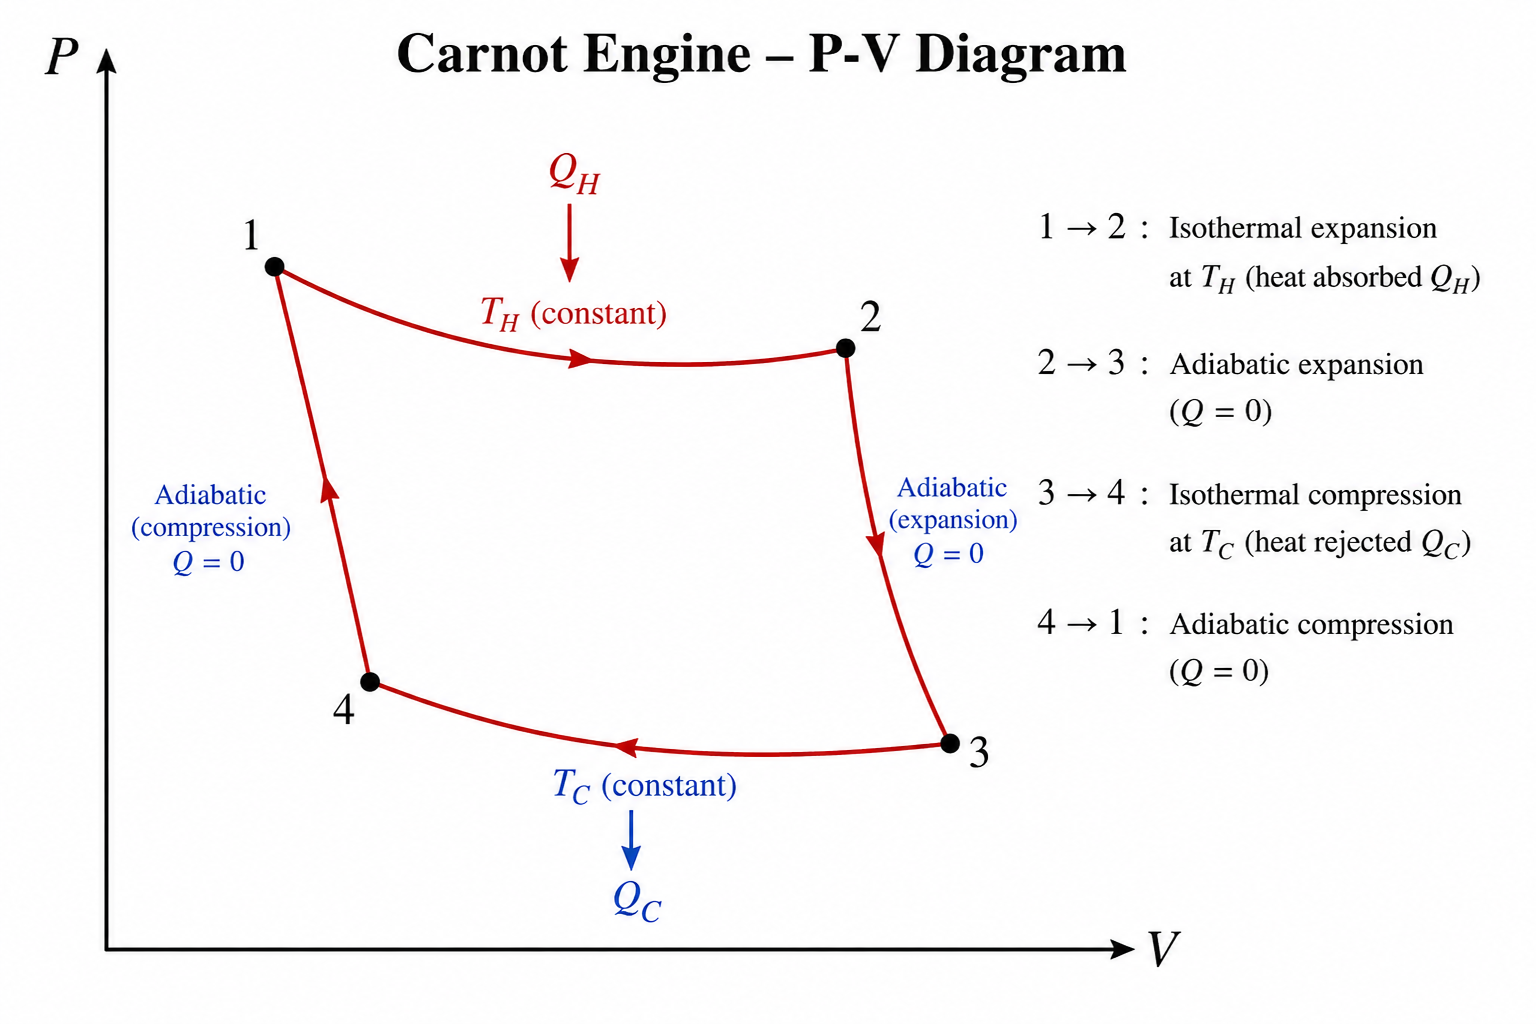
\includegraphics[width=\textwidth]{../Figure/Carnot_engine.png}
        \caption{Carnot engine.}
    \end{subfigure}
    \hfill
    \begin{subfigure}{0.45\textwidth}
        \centering
        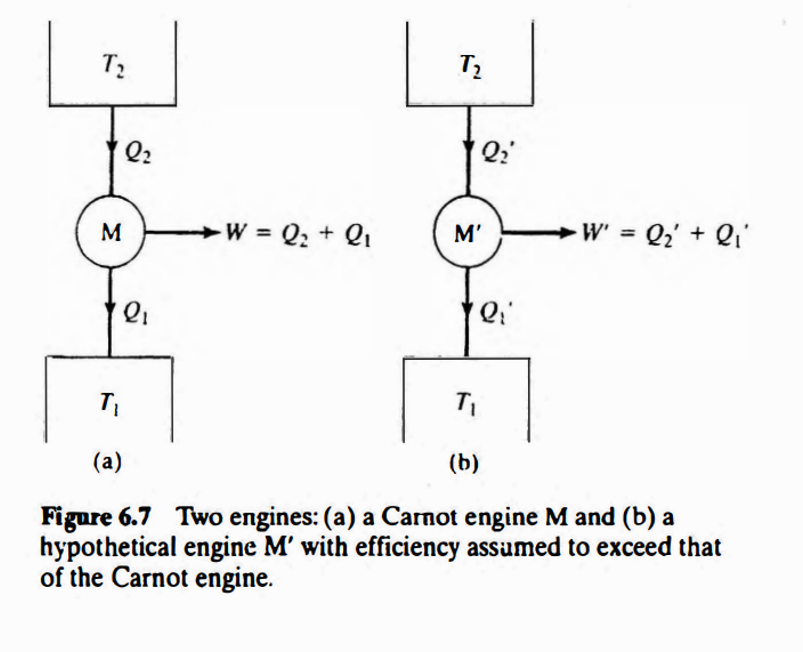
\includegraphics[width=\textwidth]{../Figure/Carnot_theorem.png}
        \caption{Diagram for proof of Carnot's theorem.}
    \end{subfigure}
\end{figure}

\begin{theorem}
\textbf{(Carnot)}All Carnot engines between the same two reservoirs have the same efficiency, regardless of the working substance. No engine can be more efficient than a Carnot engine.
\end{theorem}


\paragraph{Sketch of proof.}
Suppose there were an engine $M'$ with efficiency $e' > e_{\text{Carnot}}$. Couple $M'$ to a Carnot engine $M$ run backwards as a refrigerator, 
sized so that the work output of $M'$ exactly drives $M$. 
The net effect of the combined device is to pump a positive amount of heat from the cold reservoir to the hot reservoir with no net work 
--- a violation of the Clausius statement. Hence no such $M'$ exists. 

Note that this theorem also shows that ALL Carnot engines have the same efficiency, regardless of the substance. 
This could be shown by a similar argument: Use the engine with higher efficiency to produce work and the other one as refrigerator. 

The Carnot efficiency turns out to depend only on the two temperatures, which could be derived using ideal gas: 
\[
    e_{\text{Carnot}} = 1 - \frac{T_1}{T_2}.
\]
This relation can in fact be \emph{used} to define the absolute temperature scale: (Choose $T$ such that $\frac{Q_1}{Q_2} = \frac{T_1}{T_2}$ for a Carnot engine).

%--------------------------------------------------------------
\subsection{Clausius Inequality}
We will present a lemma that is essential for the "classical" proof of the ineqaulity using "Carnot cycle slices", 
which will not be shown here but put in the appendix. 
\begin{lemma}
For any thermodynamic substance, the internal energy and pressure are related to the absolute temperature $T$ via the modern thermodynamic equation of state:
\[
\left(\frac{\partial U}{\partial V}\right)_T + P = T\left(\frac{\partial P}{\partial T}\right)_V
\]
\end{lemma}

We will also leave the proof of the lemma to appendix as well. Now, we state the Clausius inequality: 

\begin{theorem}
    For any cyclic process, 
    \begin{enumerate}
        \item For a reversible cycle, $\displaystyle \oint \frac{\dbar Q_{\text{rev}}}{T} = 0$.
        \item For an irreversible cycle, $\displaystyle \oint \frac{\dbar Q_{\text{irr}}}{T} < 0$.
    \end{enumerate}
\end{theorem}


\begin{proof}
Let a system undergo an arbitrary, possibly irreversible, cyclic process. 
During this cycle, the system exchanges varying amounts of heat $\delta Q$ with its surroundings at varying boundary temperatures $T_{\text{ext}}$.

\textbf{1. The Setup.}

We introduce a massive master heat reservoir maintained at a constant absolute temperature $T_0$. 
We also imagine that for any value of $T_{\text{ext}}$, there exists a \textbf{reversible auxiliary Carnot engines} working between 
the master reservoir and $T_{\text{ext}}$.   

Whenever the system absorbs $\delta Q$ at $T_{\text{ext}}$, an auxiliary Carnot engine draws  $\delta Q_0$ from the master reservoir 
at $T_0$ and delivers $\delta Q$ back to $T_{\text{ext}}$ to cancel the absorption. 

Since these auxiliary engines operate completely reversibly, they strictly satisfy the absolute thermodynamic temperature ratio:
\[
\frac{\delta Q_0}{T_0} = \frac{\delta Q}{T_{\text{ext}}} \implies \delta Q_0 = T_0 \frac{\delta Q}{T_{\text{ext}}}
\]

\textbf{2. Integrating the Full Cycle.}

We allow the main system to complete one full, closed macro-cycle, returning exactly to its initial state and 
apply the First Law of Thermodynamics to the entire combined universe (consisting of the main system and all auxiliary engines). 

By conservation of energy, the total net mechanical work $W_{\text{net}}$ performed by this combined system 
must exactly equal the total net heat $Q_0$ extracted from the single master reservoir:
\[
W_{\text{net}} = Q_0 = \oint \delta Q_0
\]
Substituting our relation for $\delta Q_0$ into the cyclic integral yields:
\[
W_{\text{net}} = \oint T_0 \frac{\delta Q}{T_{\text{ext}}}= T_0 \oint \frac{\delta Q}{T_{\text{ext}}}
\]
Since the master reservoir temperature $T_0$ remains strictly constant throughout the entire process, it can be factored out of the integral. 

\textbf{3. Applying the Second Law.}  
According to the \textbf{Kelvin-Planck statement of the Second Law of Thermodynamics}, 
it is physically impossible to construct a device that operates in a cycle and produces net positive work while exchanging heat with only a single thermal reservoir. 
If the process is irreversible, the net work must be strictly less than zero. If the process is perfectly reversible, the net work is exactly zero. Thus:
\[
W_{\text{net}} \le 0
\]
Combining this constraint with our energy balance equation gives:
\[
T_0 \oint \frac{\delta Q}{T_{\text{ext}}} \le 0, \qquad \oint \frac{\delta Q}{T_{\text{ext}}} \le 0
\]
\end{proof}

\begin{center}
  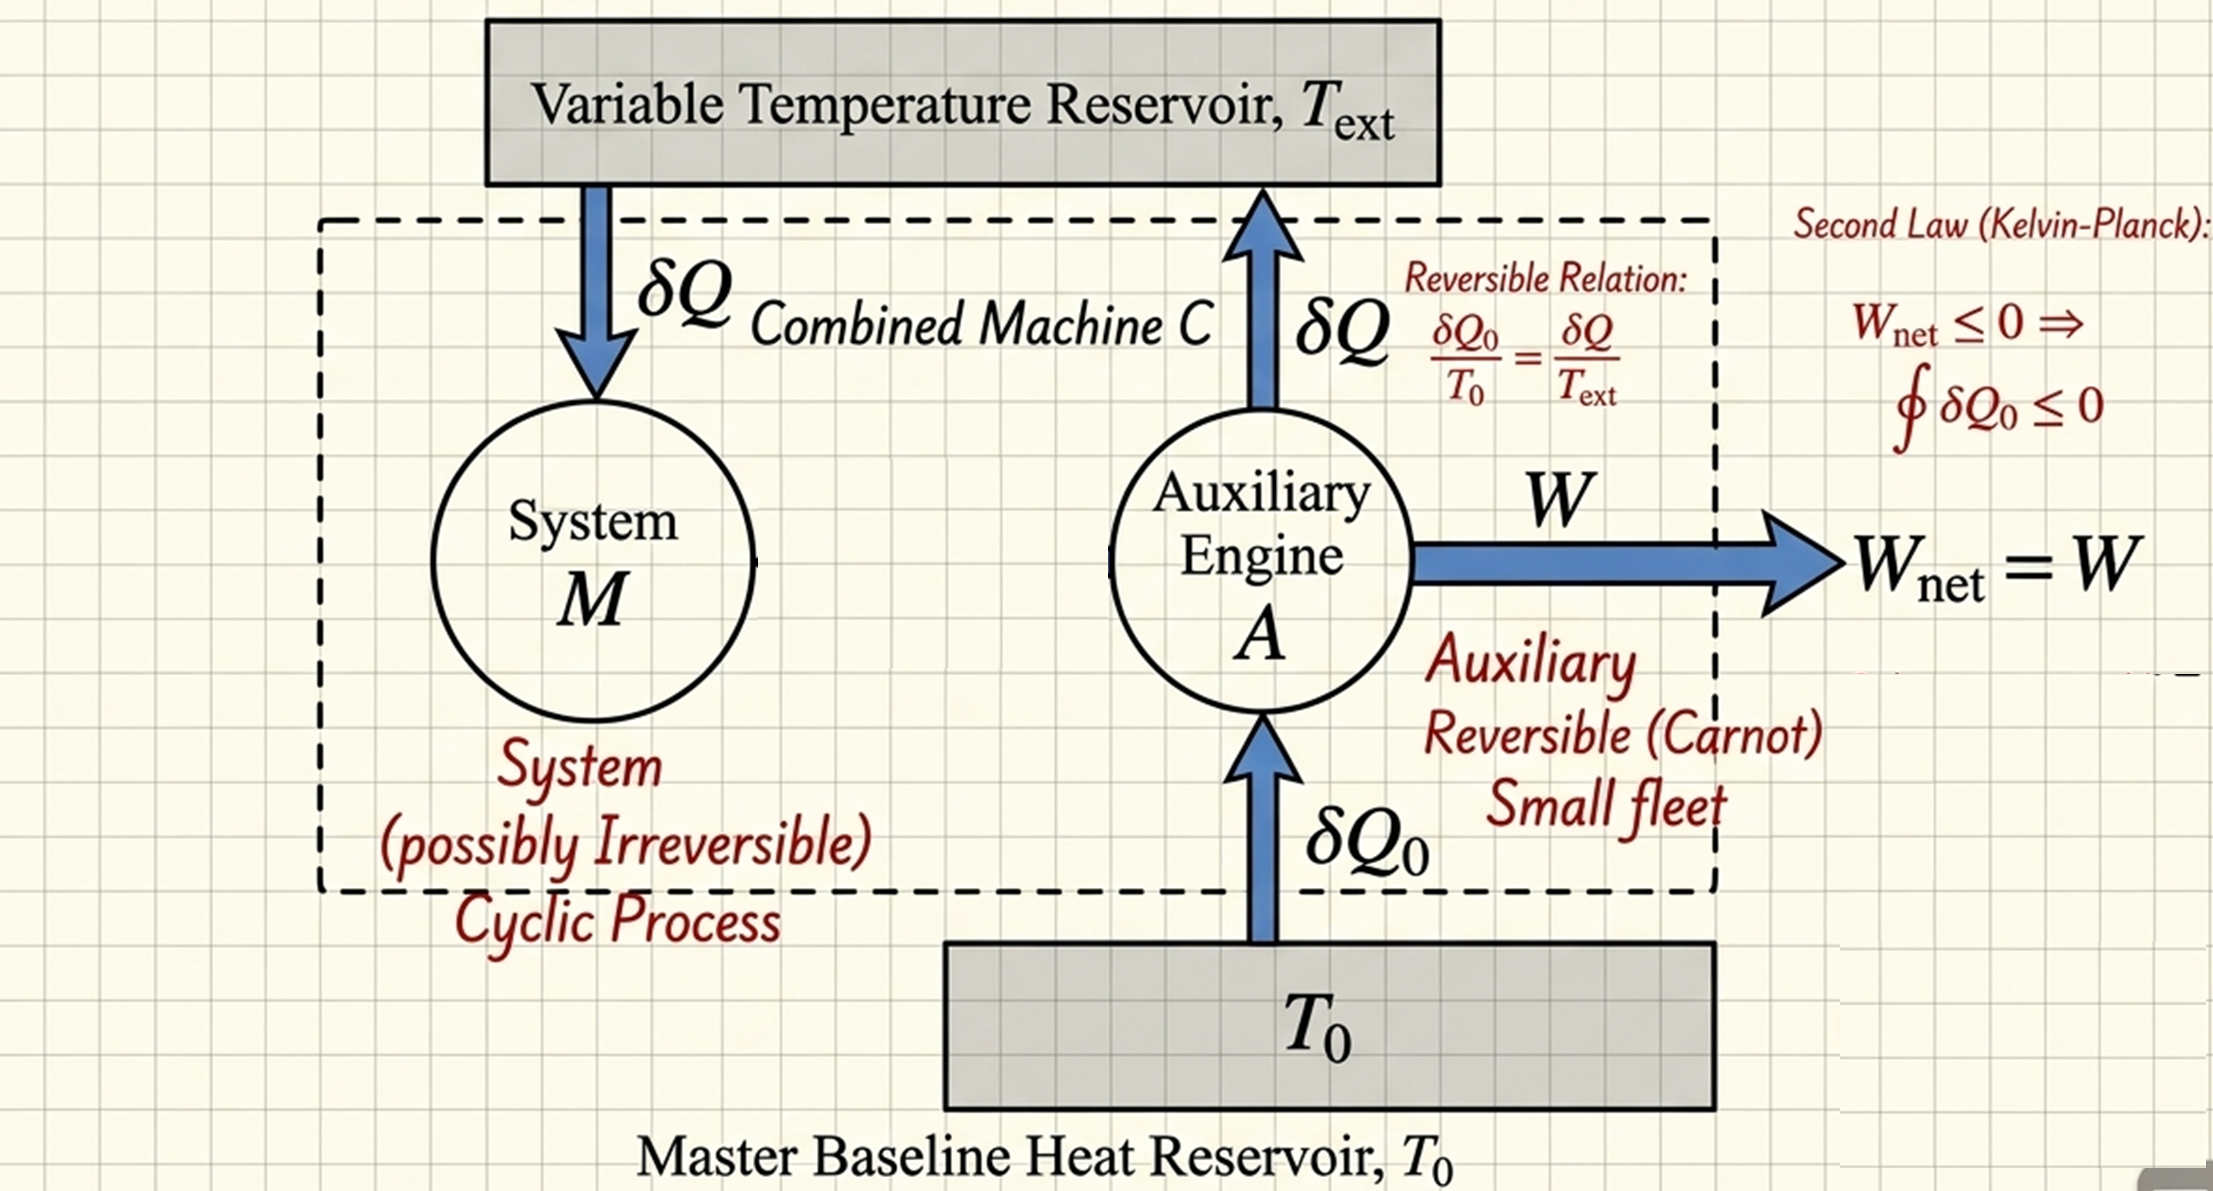
\includegraphics[width=0.8\textwidth]{../Figure/clausius_proof.png}
\end{center}


This proof actually proves both the reversible and irreversible cases. It seems that the classical "Carnot cycle slice" proof 
is actually not necessary. Nevertheless, we still present it in the appendix for completeness. See \ref{sec:clausius_inequality}.
%--------------------------------------------------------------
\subsection{Entropy}

Because $\oint \dbar Q_{\text{rev}}/T = 0$ around any closed cycle, the differential form $\dbar Q_{\text{rev}}/T$ is \emph{exact}. 
There must therefore exist a state function $S$ --- the \emph{entropy} --- whose differential is
\[
    \boxed{\,\dd S = \frac{\dbar Q_{\text{rev}}}{T}\,}.
\]
The difference $S_B - S_A$ can be computed by integrating $\dbar Q/T$ along \emph{any} reversible path from $A$ to $B$; the result is independent of the path. 
The absolute value of $S$ remains undefined at this stage, though. (it would require the Third Law, $S \to 0$ as $T \to 0$ for a perfect crystal, which we will not need here).

%==============================================================
\section{$T\dd S$ Equations}
%==============================================================
We have actually presented this lemma earlier and proved it without using the exactness in the appendix, 
but here we will provide a more elegant version using the exactness of $\dd S$, along with one corresponding to $H$. 
\subsection{A Useful Lemma from Exactness}

Entropy is a state function, so $\dd S$ is exact. Starting from
\[
    \dd S = \frac{\dbar Q}{T} = \frac{\dd U}{T} + \frac{P}{T}\,\dd V
          = \frac{C_V}{T}\,\dd T + \frac{1}{T}\!\left[P + \pa{U}{V}_T\right]\!\dd V,
\]
exactness requires that the mixed partials of the coefficients of $\dd T$ and $\dd V$ agree:
\[
    \pd{}{V}\!\left(\frac{C_V}{T}\right)_T = \pd{}{T}\!\left(\frac{1}{T}\!\left[P + \pa{U}{V}_T\right]\right)_V.
\]
Working this out and simplifying,
\[
    0 = \frac{1}{T}\!\left[\pa{P}{T}_V + \pd{^{2}U}{T\,\partial V}\right] - \frac{1}{T^{2}}\!\left(P + \pa{U}{V}_T\right),
\]
which rearranges into the very useful relation
\[
    \boxed{\,\pa{U}{V}_T = T\,\pa{P}{T}_V - P\,}.
\]
The completely analogous calculation starting from $\dd S = (\dd H - V\,\dd P)/T$ gives
\[
    \boxed{\,\pa{H}{P}_T = -T\,\pa{V}{T}_P + V\,}.
\]

\paragraph{Why these are useful.}
The two partial derivatives $\pa{U}{V}_T$ and $\pa{H}{P}_T$ were notoriously hard to compute --- Joule and Joule--Thomson told us they vanish for an ideal gas, but for solids and liquids we had no handle on them at all. With these lemmas, all we need are the \emph{measurable} mechanical responses: the thermal expansion coefficient $\beta = \pa{V}{T}_P/V$ and the pressure--temperature derivative $\pa{P}{T}_V$. Both are routine tabletop measurements.

\paragraph{Exercise.}
\zh{
(A) 卡諾熱機在兩個不同溫度的熱庫（heat reservoir）循環運作時，其過程均為可逆。

考慮如圖 1 所示的卡諾熱機，熱機由二可逆等溫過程（$a \to b$；$c \to d$）和二可逆絕熱過程（$b \to c$；$d \to a$）組成。
試計算每一過程中熱機內氣體（假設為 $n$ 莫耳的理想氣體）熵的變化量。

（以氣體壓力 $P$、體積 $V$、溫度 $T$ 和其他相關常數表示。）（8 分）

(B) 現考慮兩個具有相同熱容量 $C$ 的物質，其起始溫度分別為 $T_1$ 和 $T_2$。今有一卡諾熱機

以此二物質為其低溫和高溫熱庫，並假設卡諾熱機運行一循環時，二熱庫的溫度變化，

遠小於其個別的溫度值。

問此二物質的最終溫度為何？過程中卡諾熱機可作的最大功為何？（9 分）

(C) 現考慮三個具有相同熱容量 $C$ 的物質，其起始溫度分別為
$T_1 = 100\,\mathrm{K}$、
$T_2 = 300\,\mathrm{K}$
和
$T_3 = 300\,\mathrm{K}$。

假設我們可以利用前述的卡諾熱機在物質 1 和 2 之間運轉並輸出功，並以另一在物質 1 和物質 3 之間運轉的卡諾熱機，將所輸出的功完全用於提高物質 3 的溫度。問：

(i) 物質 1 所能達到的最低溫度 $T_L$ 為何？（2 分）

(ii) 物質 3 可以達到的最高溫度 $T_H$ 為何？（6 分）
}
\paragraph{Solution.}
\textbf{(A)} \\
In a Carnot cycle, all 4 processes are reversible. Thus, the entropy change $\Delta S$ of the gas in each step is given by:
\[ \Delta S = \int_{i}^{f} \frac{dQ}{T} \]
For the adiabatic processes ($b \to c$ and $d \to a$):
\[ \Delta S_{b \to c} = 0, \quad \Delta S_{d \to a} = 0 \quad (\text{since } dQ = 0) \]
For the isothermal processes ($a \to b$ and $c \to d$):
\[ dQ = dU + P\,dV = P\,dV = \frac{nRT}{V}\,dV \]
\[ \Rightarrow \Delta S = \int_{V_i}^{V_f} \frac{nRT}{TV}\,dV = nR \ln \frac{V_f}{V_i} \]
Thus,
\[ \Delta S_{a \to b} = nR \ln \frac{V_b}{V_a}, \quad \Delta S_{c \to d} = nR \ln \frac{V_d}{V_c} \]
Note that by the properties of an adiabatic process ($TV^{\gamma-1} = \text{const}$), we have:
\begin{align*}
T_H V_a^{\gamma-1} &= T_L V_d^{\gamma-1} \\
T_H V_b^{\gamma-1} &= T_L V_c^{\gamma-1}
\end{align*}
Dividing the two equations yields:
\[ \left(\frac{V_a}{V_b}\right)^{\gamma-1} = \left(\frac{V_d}{V_c}\right)^{\gamma-1} \implies \frac{V_a}{V_b} = \frac{V_d}{V_c} \implies \frac{V_b}{V_a} = \frac{V_c}{V_d} \]
Therefore, the entropy change in the second isothermal process is:
\[ \Delta S_{c \to d} = nR \ln \frac{V_d}{V_c} = -nR \ln \frac{V_c}{V_d} = -nR \ln \frac{V_b}{V_a} = -\Delta S_{a \to b} \]
(This is consistent with the fact that $S$ is a state variable, so $\Delta S_{\text{cycle}} = 0$.)

\vspace{1em}
\textbf{(B)} \\
Let the initial temperatures of the two reservoirs be $T_{1,i}$ and $T_{2,i}$ with $T_{2,i} > T_{1,i}$. Let $\rho = \frac{V_b}{V_a}$ be the expansion ratio. 
For an infinitesimal cycle, the heat exchanged with the reservoirs is:
\[ dQ_{\text{hot}} = -dQ_{a \to b} \implies C\,dT_2 = -nR T_2 \ln \rho \]
\[ dQ_{\text{cold}} = dQ_{c \to d, \text{rejected}} \implies C\,dT_1 = nR T_1 \ln \rho \]
Rearranging these gives:
\[ -\frac{dT_2}{T_2} = \frac{nR}{C}\ln \rho = \frac{dT_1}{T_1} \]
Integrating over many cycles until the final equilibrium state $T_{1,f} = T_{2,f} = T_f$:
\[ \int_{T_{1,i}}^{T_f} \frac{dT_1}{T_1} = -\int_{T_{2,i}}^{T_f} \frac{dT_2}{T_2} \]
\[ \Rightarrow \ln \frac{T_f}{T_{1,i}} = -\ln \frac{T_f}{T_{2,i}} = \ln \frac{T_{2,i}}{T_f} \]
\[ \Rightarrow T_f^2 = T_{1,i} T_{2,i} \implies T_f = \sqrt{T_{1,i} T_{2,i}} \]
(Using the parameters from the problem statement, the final temperature is $\sqrt{T_1 T_2}$.)

The maximum work $W$ done by the engine can be found using energy conservation ($W = -\Delta U_{\text{reservoirs}}$):
\begin{align*}
W &= -C(T_f - T_{2,i}) - C(T_f - T_{1,i}) \\
  &= C(T_{1,i} + T_{2,i} - 2T_f) \\
  &= C\left(T_{1,i} + T_{2,i} - 2\sqrt{T_{1,i}T_{2,i}}\right) = C\left(\sqrt{T_{2,i}} - \sqrt{T_{1,i}}\right)^2
\end{align*}

\vspace{1em}
\textbf{(C)} \\
Let Engine 1 operate between $T_2$ and $T_1$, extracting heat $Q_h$ from $T_2$, rejecting heat to $T_1$, and producing work $W = \eta_1 Q_h$.
Let Engine 2 (acting as a heat pump) operate between $T_1$ and $T_3$, using all the work $W$ to pump heat from $T_1$ to $T_3$. The coefficient of performance is $1/\eta_2$.
Heat delivered to $T_3$ is $Q_3 = W/\eta_2 = (\eta_1/\eta_2)Q_h$.
Heat extracted from $T_1$ by the pump is $Q_{\text{extracted}} = Q_3 - W = \eta_1\left(\frac{1}{\eta_2}-1\right)Q_h$.

\textbf{(i)} The net heat added to substance 1 is:
\[ dQ_1 = (1-\eta_1)Q_h - \eta_1\left(\frac{1}{\eta_2}-1\right)Q_h = \left(1 - \frac{\eta_1}{\eta_2}\right)Q_h \]
Since $T_2 \downarrow$ and $T_3 \uparrow$, we have $\eta_1 \downarrow$ and $\eta_2 \uparrow$. Initially $T_2 = T_3 = 300\,\text{K}$, so $\eta_1 = \eta_2$.
As the process proceeds, $\eta_1 \le \eta_2$, which implies $1 - \frac{\eta_1}{\eta_2} \ge 0$.
Thus, $dQ_1 \ge 0$. Since heat is continuously added to substance 1, its temperature never decreases.
Therefore, the minimum temperature is its initial temperature:
\[ T_{1,\text{min}} = 100\,\text{K} \]

\textbf{(ii)} For the system of three substances, assuming all processes are reversible, the total entropy change is zero:
\[ dS_1 + dS_2 + dS_3 = \frac{dQ_1}{T_1} + \frac{dQ_2}{T_2} + \frac{dQ_3}{T_3} = 0 \]
\[ \Rightarrow C\left(\frac{dT_1}{T_1} + \frac{dT_2}{T_2} + \frac{dT_3}{T_3}\right) = 0 \implies d(\ln(T_1 T_2 T_3)) = 0 \]
\[ \Rightarrow T_1 T_2 T_3 = \text{const} = 100 \times 300 \times 300 = 9 \times 10^6 \]
By energy conservation, no net heat or work is exchanged with the environment:
\[ dQ_1 + dQ_2 + dQ_3 = 0 \implies C(dT_1 + dT_2 + dT_3) = 0 \]
\[ \Rightarrow T_1 + T_2 + T_3 = \text{const} = 100 + 300 + 300 = 700 \]
To maximize $T_3$, $T_2$ must decrease until Engine 1 can no longer extract work, which happens when $T_1 = T_2 = T$.
Substitute $T_1 = T_2 = T$ into the conservation equations:
\[ 2T + T_3 = 700 \implies T_3 = 700 - 2T \]
\[ T^2 T_3 = 9 \times 10^6 \implies T^2(700 - 2T) = 9 \times 10^6 \]
\[ 2T^3 - 700T^2 + 9 \times 10^6 = 0 \implies T^3 - 350T^2 + 4.5 \times 10^6 = 0 \]
By inspection, $T = 150\,\text{K}$ is a root ($150^3 - 350(150^2) + 4.5 \times 10^6 = 3375000 - 7875000 + 4500000 = 0$).
Therefore, $T_3 = 700 - 2(150) = 400\,\text{K}$.
The maximum temperature that substance 3 can reach is:
\[ T_H = 400\,\text{K} \]

%--------------------------------------------------------------
\subsection{The Three $T\dd S$ Equations}

We can compute $\dd S$ as a function of any two of $P,V,T$. There are three pairs, hence three forms:
\begin{align}
    T\,\dd S &= n C_V\,\dd T + T\,\pa{P}{T}_V\,\dd V, \label{eq:TdS1}\\[4pt]
    T\,\dd S &= n C_P\,\dd T - T\,\pa{V}{T}_P\,\dd P, \label{eq:TdS2}\\[4pt]
    T\,\dd S &= n C_P\,\pa{T}{V}_P\,\dd V + n C_V\,\pa{T}{P}_V\,\dd P. \label{eq:TdS3}
\end{align}
The derivations are straightforward: write $\dbar Q = T\,\dd S$ in the First Law, then use whichever pair of $(P,V,T)$ you wish as the free variables (the third one is eliminated via the equation of state and the lemma above).

\paragraph{Application: entropy change of an ideal gas.}
Substituting $\pa{P}{T}_V = nR/V$ into~\eqref{eq:TdS1},
\[
    T\,\dd S = n C_V\,\dd T + \frac{nRT}{V}\,\dd V.
\]
Dividing through by $T$ and integrating (a slightly informal step: we are assuming $C_V$ is constant, which is fine for monatomic and diatomic ideal gases in the IPhO range),
\[
    \boxed{\,\Delta S = n C_V \ln\!\frac{T}{T_0} + nR \ln\!\frac{V}{V_0}\,}.
\]
This formula is the workhorse of olympiad entropy problems. Note that it is for an ideal gas only.


%==============================================================
\section{Thermodynamic Potentials}
%==============================================================

\subsection{The Four Energies}

We have already met two state functions with units of energy, $U$ and $H$. We now introduce two more:
\begin{align*}
    A &\equiv U - TS \qquad \text{(Helmholtz free energy)},\\
    G &\equiv H - TS \qquad \text{(Gibbs free energy)}.
\end{align*}
All four are state functions, and their differentials (after substituting $\dbar Q_{\text{rev}}=T\,\dd S$ and $\dbar W_{\text{rev}}=-P\,\dd V$) are
\[
    \boxed{\begin{aligned}
        \dd U &= T\,\dd S - P\,\dd V, \vphantom{\left(\frac{\partial U}{\partial S}\right)_V} \\
        \dd H &= T\,\dd S + V\,\dd P, \vphantom{\left(\frac{\partial H}{\partial S}\right)_P} \\
        \dd A &= -S\,\dd T - P\,\dd V, \vphantom{\left(\frac{\partial A}{\partial T}\right)_V} \\
        \dd G &= -S\,\dd T + V\,\dd P, \vphantom{\left(\frac{\partial G}{\partial T}\right)_P}
    \end{aligned}}
    \quad\implies\quad
    \begin{aligned}
        \left(\frac{\partial U}{\partial S}\right)_V &= T, & \left(\frac{\partial U}{\partial V}\right)_S &= -P, \\[1ex]
        \left(\frac{\partial H}{\partial S}\right)_P &= T, & \left(\frac{\partial H}{\partial P}\right)_S &= V, \\[1ex]
        \left(\frac{\partial A}{\partial T}\right)_V &= -S, & \left(\frac{\partial A}{\partial V}\right)_T &= -P, \\[1ex]
        \left(\frac{\partial G}{\partial T}\right)_P &= -S, & \left(\frac{\partial G}{\partial P}\right)_T &= V.
    \end{aligned}
\]
Note that we could "read off" the coefficients like this because now the differentials are exact, unlike the original $\dd U = \dbar Q + \dbar W$.
Read each formula off the variables on its right-hand side: $U(S,V)$, $H(S,P)$, $A(T,V)$, $G(T,P)$. 
Althought now we have four variables, $\{P,V,T,S\}$, the degree of freedom is still 2. 

\paragraph{Why introduce $A$ and $G$?}
\begin{itemize}
    \item $A$ is minimised at equilibrium when $T$ and $V$ are held fixed 
    \item $G$ is minimised at equilibrium when $T$ and $P$ are held fixed
\end{itemize}

%--------------------------------------------------------------
\subsection{Maxwell Relations}

Each of the four potentials is a state function, so each of their differentials is exact, and the mixed partial derivatives of any two coefficients are equal. From $\dd U = T\,\dd S - P\,\dd V$, for instance,
\[
    \pa{T}{V}_S = -\pa{P}{S}_V.
\]
Doing this for all four potentials gives the four \emph{Maxwell relations}:
\[
    \boxed{\begin{aligned}
        \pa{T}{V}_S &= -\pa{P}{S}_V \qquad (\text{from } \dd U),\\[4pt]
        \pa{T}{P}_S &= \phantom{-}\pa{V}{S}_P \qquad (\text{from } \dd H),\\[4pt]
        \pa{S}{V}_T &= \phantom{-}\pa{P}{T}_V \qquad (\text{from } \dd A),\\[4pt]
        \pa{S}{P}_T &= -\pa{V}{T}_P \qquad (\text{from } \dd G).
    \end{aligned}}
\]
The last two are by far the most useful in problem solving --- you will see them appear in essentially every $T\dd S$ computation.

%==============================================================
\section{Multi-phase and Multi-species Systems}
%==============================================================

\subsection{Adding Composition Variables}

So far each system has been a single phase with a single chemical species. Once we allow more, the variable count goes up: with two phases (say liquid and vapour of the same substance) the total mole number $n_1 + n_2$ is fixed, but the split between phases is a new degree of freedom.

Using $G$ as an example, for a two-phase system,
\[
    \dd G = -S\,\dd T + V\,\dd P + \pa{G}{n_1}_{T,P,n_2}\dd n_1 + \pa{G}{n_2}_{T,P,n_1}\dd n_2.
\]
Because the total $n_1 + n_2$ is conserved, $\dd n_2 = -\dd n_1$, and the last two terms combine into
\[
    \dd G = -S\,\dd T + V\,\dd P + (\mu_1 - \mu_2)\,\dd n_1,
\]
where
\[
    \mu_i \equiv \pa{G}{n_i}_{T,P,n_{j\neq i}}
\]
is the \emph{chemical potential} of species (or phase) $i$. The chemical potential is the change in $G$ per mole of $i$ added at fixed $T,P$ and other species.

%--------------------------------------------------------------
\subsection{Gibbs Energy and Spontaneity}

We now justify the standard chemistry-textbook claim:
\begin{quote}
\textit{At constant $T$ and $P$, a spontaneous process satisfies $\Delta G < 0$.}
\end{quote}

\paragraph{Setup.} Consider a closed system in thermal and mechanical contact with surroundings at fixed $T$ and $P$. Suppose a process absorbs heat $\Delta Q$ from the surroundings. The surroundings, being large, change reversibly, so their entropy change is
\[
    \Delta S_{\text{sur}} = -\frac{\Delta Q}{T}.
\]
\paragraph{First law for the system.} Assuming the work is purely $PV$-work and the system path can be made reversible,
\[
    \Delta Q = \Delta U + P\,\Delta V.
\]
\paragraph{Clausius for the imagined return.} Now imagine running a (hypothetical) reversible process that brings the system back to its initial state. By the Clausius inequality applied to the irreversible cycle (forward irreversible + reverse reversible),
\[
    \Delta Q < T\,\Delta S_{\text{sys}}.
\]
(Equality holds iff the forward step was already reversible.)

\paragraph{Putting it together.} Combine the two:
\[
    \Delta U + P\,\Delta V < T\,\Delta S
    \;\;\Longleftrightarrow\;\;
    \Delta U + P\,\Delta V - T\,\Delta S < 0
    \;\;\Longleftrightarrow\;\;
    \Delta(U + PV - TS) < 0,
\]
where in the last step we used that $T$ and $P$ are held constant. The combination $U + PV - TS$ is precisely $G$, so
\[
    \boxed{\,\Delta G < 0\,}
\]
for any spontaneous process at constant $T$ and $P$, with $\Delta G = 0$ at equilibrium.

%==============================================================
\section{Phase Equilibrium and the Clapeyron Equation}
%==============================================================

\subsection{The Clapeyron Equation}

Consider two phases ($1$ = liquid, $2$ = vapour, say) of the same substance coexisting at some temperature $T$ and pressure $P$. Let $n_1,n_2$ be the mole numbers of the two phases, with $n_1+n_2$ fixed. If a small amount $-\dd n_1 = \dd n_2 > 0$ converts phase~$1$ into phase~$2$, the Gibbs energy changes by
\[
    \dd G = (\mu_2 - \mu_1)\,\dd n_1.
\]
At equilibrium $\dd G = 0$ for arbitrary $\dd n_1$, which forces
\[
    \boxed{\,\mu_1(T,P) = \mu_2(T,P)\,}.
\]
This is the \emph{phase equilibrium condition}: across the coexistence curve in the $(T,P)$ plane, the chemical potentials of the two phases are equal.

\paragraph{Sliding along the coexistence curve.}
Now suppose we change $T\to T+\dd T$ and $P\to P+\dd P$ in such a way that the two phases continue to coexist. Then $\mu_1=\mu_2$ must persist, i.e.\ $\dd\mu_1=\dd\mu_2$. Using the molar versions of $\dd G = -S\,\dd T + V\,\dd P$,
\[
    \dd\mu_1 = -s_1\,\dd T + v_1\,\dd P
    = -s_2\,\dd T + v_2\,\dd P
    = \dd\mu_2,
\]
where lowercase $s_i, v_i$ are the molar entropy and molar volume of phase $i$. Solving for $\dd P/\dd T$,
\[
    \boxed{\,\frac{\dd P}{\dd T} = \frac{s_2 - s_1}{v_2 - v_1} = \frac{\Delta H_{\text{trans}}}{T\,\Delta v}\,}.
\]
The last equality uses $T\,\Delta s = \Delta H_{\text{trans}}$, the molar latent heat of the transition (valid because the transition occurs at constant $T$ and $P$). This is the \textbf{Clapeyron equation}.

%--------------------------------------------------------------
\subsection{The Clausius--Clapeyron Equation}

For the liquid--vapour transition, we make two further approximations:
\begin{enumerate}[label=(\roman*)]
    \item the vapour behaves as an ideal gas, so $v_{\text{vap}} = RT/P$;
    \item the vapour volume vastly exceeds the liquid volume, so $\Delta v \approx v_{\text{vap}}$.
\end{enumerate}
Substituting into the Clapeyron equation,
\[
    \frac{\dd P}{\dd T} = \frac{\Delta H}{T\,(RT/P)} = \frac{\Delta H}{R}\,\frac{P}{T^{2}}.
\]
Separating variables and integrating (assuming $\Delta H$ approximately constant over the temperature range),
\[
    \int_{P_0}^{P} \frac{\dd P'}{P'} = \frac{\Delta H}{R}\int_{T_0}^{T} \frac{\dd T'}{T'^{2}}
    \;\;\Longrightarrow\;\;
    \boxed{\,\ln\!\frac{P}{P_0} = -\frac{\Delta H}{R}\!\left(\frac{1}{T} - \frac{1}{T_0}\right)\,},
\]
or in exponentiated form,
\[
    P = P_0 \exp\!\left[-\frac{\Delta H}{R}\!\left(\frac{1}{T} - \frac{1}{T_0}\right)\right].
\]
This is the \textbf{Clausius--Clapeyron equation}. 
% =============================================================
%  End of classical_thermodynamics.tex
% =============================================================

\chapter{Statistical Thermodynamics}

\noindent\textit{Reference: R.K. Pathria, P.D. Beele. \emph{Statistical Mechanics}, Chapters~1--8.}
\section{Microcanonical ensemble}
\paragraph{Macrostates and macrostates.}
\begin{enumerate}
    \item \textbf{Macrostate:} In microcanonical ensemble, the macrostate is specified by $N,V,E$.
    \item \textbf{Microstate:} Classically, it's represented by the positions and momenta of all particles (phase space), while quantum mechanically it's represented by the number of particles occupying each energy level, etc.
\end{enumerate}

\paragraph{Postulates.}
\begin{enumerate}[label=(\arabic*)]
    \item All microstates are equally probable.
    \item The system is in equilibrium $\iff$ the system is in the macrostate where the number of microstates is maximized.
\end{enumerate}

\textcolor{blue}{Q: How do we define "1 microstate" classically when the phase space is continuous?}
\textbf{Ans}: One microstate $= h^{k} = h^{3N}$, where $k=3N$ is the number of degrees of freedom. 
Check Pathria Chapter 2 for details. 

\begin{definition}[Statistical temperature]
The statistical temperature $\beta$ is defined as
\[
    \beta = \left(\frac{\partial(\ln\Omega(N,V,E))}{\partial E}\right)_{N,V}.
\]
\end{definition}

\begin{theorem}
Two systems are in equilibrium only if their $\beta$ are equal.
\end{theorem}

\begin{proof}
Consider two systems that could exchange energies, with $N_i,V_i$ fixed.
Total energy $E_0 = E_1+E_2 = \mathrm{const}$.
The total number of microstates is
\[
    \Omega(E_0,E_1) = \Omega_1(E_1)\,\Omega_2(E_0-E_1).
\]
Maximum condition: when $E_1 = \E_1$, the corresponding $\E_2 = E_0-\E_1$ satisfies
\[
    \frac{\partial\Omega_1}{\partial E_1}(\E_1)\,\Omega_2(\E_2) - \Omega_1(\E_1)\frac{\partial\Omega_2}{\partial E_2}(\E_2) = 0.
\]
Hence
\[
    \frac{\partial(\ln\Omega_1)}{\partial E_1} = \frac{\partial(\ln\Omega_2)}{\partial E_2}
    \quad\Longrightarrow\quad \beta_1 = \beta_2. \qedhere
\]
\end{proof}

\begin{framed}
    \textbf{Postulate.} Planck assumes: 
    \[
        S = k\ln\Omega,
    \]
\end{framed}
If this is true, in thermodynamics we have $\bigl(\frac{\partial S}{\partial E}\bigr)_{N,V} = \frac{1}{T}$, we then have $k\beta = \tfrac{1}{T}$, or $\beta = \tfrac{1}{kT}$.

\begin{remark}
    ...
    \begin{itemize}
        \item Planck probably get this idea in reverse: He first noticed that $\bigl(\frac{\partial S}{\partial E}\bigr)_{N,V} = \frac{1}{T}$, and then figured out $S = k\ln\Omega$ might make sense. 
        \item We have not confirmed the $k$ is indeed $k_B$ yet. We will see that this is indeed the case when we apply the postulates to ideal gas.
    \end{itemize}
\end{remark}

\textbf{\textcolor{blue}{Q: How do we confirm that $S=k\ln\Omega$ is correct?}}

\textbf{Ans:} We define statistical $S$ using an inspiration, and then imitate classical thermodynamics to define $T,P,C_v,$ etc. 
Using ideal gas as example (see next subsection), we then find that $PV=NkT$, $C_V=\frac{3}{2}NkT$ etc., supporting this guess.

\begin{proposition}
If the volume of two systems can be changed, then not only do we need $T_1=T_2$ (i.e.\ $\beta_1=\beta_2$), but also
\[
    \eta_1 = \eta_2,\qquad \text{where } \eta = \left(\frac{\partial\ln\Omega}{\partial V}\right)_{N,E}\bigg|_{V=\bar V}.
\]
\end{proposition}

\begin{proof}
Same as the $\beta$ case.
\end{proof}

\begin{proposition}
Given $S=k\ln\Omega$ and $T\,dS = dE + P\,dV - \mu\,dN$, we have
\[
    \eta = \frac{P}{kT}.
\]
On the other hand, if $\zeta = \left(\frac{\partial\ln\Omega}{\partial N}\right)_{V,E}\big|_{N=\N}$, then
\[
    \zeta = -\frac{\mu}{kT}.
\]
\end{proposition}

\subsection{Example: Ideal Gas}

\paragraph{I. Ideal-gas Law.}
With merely the fact that $\Omega(N,E,V)\propto V^{N}$, we could already have:
\[
    \frac{P}{kT} = \frac{N}{V} \quad\Longrightarrow\quad PV = NkT.
\]
We could see that $k$ is indeed $k_B$ we are used to.

\paragraph{II. Monatomic Ideal Gas in Adiabatic Reversible Process.}
The energy of a single atom (in a box) can be written as
\[
    \varepsilon = \frac{h^{2}}{8mV^{2/3}}\,(n_x^{2}+n_y^{2}+n_z^{2}).
\]
Therefore $\Omega(N,E,V)$ is simply the number of possible sets of $(n_x,n_y,n_z)$ that satisfy the equation above. For $\Omega(N,E,V)$, the equation is naturally also just
\[
    \sum_{i=1}^{3N} n_i^{2} = \frac{8m V^{2/3} E}{h^{2}} \equiv E^{*}.
\]
From this we infer that $S(N,E,V) = S(N,\lambda(E,V))$.
Therefore, when $S$ and $N$ are constant (reversible adiabatic),
\[
    V^{2/3}E = \mathrm{const} \xRightarrow{P=\frac{2}{3}\frac{E}{V}} P V^{5/3} = \mathrm{const}.
\]

\paragraph{III. Actual Number of Microstates and Specific Heat (Distinguishable).}
Consider first $\Sigma(N,\lambda<E^{*})$, the number of points within the ``positive compartment'' of a $3N$-sphere (just like we divide by $\frac{1}{8}$ in the 1-particle case):
\[
    \Sigma(N,\lambda<E^{*}) \approx \left(\frac{1}{2}\right)^{N}\frac{\pi^{3N/2}}{(3N/2)!}\,(E^{*})^{3N/2}
    = \left(\frac{V}{h^{3}}\right)^{N}\frac{(2\pi m E)^{3N/2}}{(3N/2)!}.
\]
To obtain $\Omega(N,V,E)$ (or, more practically, $\Omega(N,V, E\le E^{*}<E+\Delta)$) we need
\[
    \Omega(N,V,E,\Delta) \approx \frac{\partial\Sigma}{\partial E}\Delta \approx \frac{3N}{2}\Sigma\Delta.
\]
So
\[
    \boxed{\ln\Omega \approx N\ln\!\left[\frac{V}{h^{3}}\!\left(\frac{2\pi mE}{3N}\right)^{3/2}\right] + \frac{3}{2}N + O(\ln N).}
\]
Using $S=k\ln\Omega$:
\[
    E(S,V,N) = \frac{3 h^{2} N}{4\pi m V^{2/3}}\exp\!\left(\frac{2S}{3Nk}-1\right).
\]
By $\bigl(\frac{\partial E}{\partial S}\bigr)_{N,V} = T$:
\[
    E(S,V,N) = \tfrac{3}{2} N k T(S,V,N), \qquad
    \left(\frac{\partial E}{\partial T}\right)_{N,V} = \boxed{C_V = \tfrac{3}{2} N k}.
\]

\subsection{Example}

\zh{波茲曼在19世紀末提出下列猜想：}$S=k \ln \Omega$\zh{，這裡 } $S$ \zh{是熵，}$k$\zh{ 是波茲曼常數，則 }$\Omega$\zh{ 為系統狀態數。考慮 }$N$\zh{ 個單原子分子組成的理想氣體，其內能}
\[ U=\sum_{j=1}^{N}\frac{|\vec{p}_{j}|^{2}}{2m} \]
\zh{，這裡 }$m$\zh{ 是氣體分子的質量，}$\vec{p}_{j}$\zh{ 是第 }$j$\zh{ 個氣體分子的動量。}

\zh{若不考慮全同粒子效應則 }$\Omega=\Omega_{1}=\prod_{j=1}^{N}\int\frac{d^{3}x_{j}d^{3}p_{j}}{h^{3}}=\left(\frac{V}{h^{3}}\right)^{N}A_{3N-1}(\sqrt{2mU})$\zh{，這裡 }$d^{3}x_{j}d^{3}p_{j}$\zh{ 是第 }$j$\zh{ 個氣體分子的相空間體積，}$V$\zh{ 為系統體積，}$h$\zh{ 是普朗克常數，}$A_{n-1}(R)$\zh{ 代表半徑為 }$R$\text{、}$n-1$\zh{ 維球 }$x_{1}^{2}+x_{2}^{2}+\dots+x_{n}^{2}=R^{2}$\zh{ 的表面積，例如當 }$n=2$\zh{ 時，}$A_{1}(R)=2\pi R$\zh{；當 }$n=3$\zh{ 時，}$A_{2}(R)=4\pi R^{2}$\zh{；可得}
\[ A_{n-1}(R)=\frac{2(\pi^{n/2})}{\Gamma(\frac{n}{2})}R^{n-1} \]
\zh{，其中 Gamma 函數 }$\Gamma(z)=\int_{0}^{\infty}x^{z-1}e^{-x}dx$\zh{。}

\zh{若考慮全同粒子效應則 }$\Omega=\Omega_{2}=\frac{1}{N!}\prod_{j=1}^{N}\int\frac{d^{3}x_{j}d^{3}p_{j}}{h^{3}}=\frac{1}{N!}\Omega_{1}$。\zh{在本題中，我們要利用理想氣體系統驗證波茲曼猜想的正確性，且考慮全同粒子效應可以解決 Gibbs paradox。}

\vspace{1.5em}
\subsection*{\zh{問題}}

\textbf{(A)} \zh{考慮 }$N \gg 1$\zh{ 的極限，利用史特靈近似：當 }$z$\zh{ 為正整數且 }$z \gg 1$\zh{ 時，}$\Gamma(z+1)=z! \approx e^{-z}z^{z}$\zh{，證明用 }$\Omega_{1}$\zh{ 及 }$\Omega_{2}$\zh{ 所求得的熵分別為}
\begin{align*}
S_{1}&=k \ln \Omega_{1} \approx Nk\left\{\ln\left[V\left(\frac{4\pi mU}{3h^{2}N}\right)^{3/2}\right]+\frac{3}{2}\right\} \\
S_{2}&=k \ln \Omega_{2} \approx Nk\left\{\ln\left[\frac{V}{N}\left(\frac{4\pi mU}{3h^{2}N}\right)^{3/2}\right]+\frac{5}{2}\right\}
\end{align*}
\zh{若已知內能 }$U$\zh{ 滿足等式 }$dU=TdS-PdV+\mu dN$\zh{，這裡 }$T, P, \mu$\zh{ 為系統的溫度、壓力及化學勢（當系統的熵及體積為不變時，在系統中增加一個粒子所需耗費的能量）。這個等式意味著我們應該將 }$U, T, P, \mu$\zh{ 等物理量視為 }$S, V, N$\zh{ 的函數，即：}
\[ U=U(S,V,N), \quad T=T(S,V,N), \quad P=P(S,V,N), \quad \mu=\mu(S,V,N) \]

\vspace{0.5em}
\textbf{(B)} \zh{利用 (A) 小題的結果，由 }$S_{1}$\zh{ 或 }$S_{2}$\zh{ 求出單原子分子理想氣體的內能 }$U$\zh{，並證明理想氣體狀態方程式 }$PV=NkT$\zh{。}

\vspace{0.5em}
\textbf{(C)} \zh{利用 (A)(B) 小題的結果，由 }$S_{1}$\zh{ 或 }$S_{2}$\zh{ 求理想氣體對應的化學勢 }$\mu_{1}, \mu_{2}$\zh{，以 }$T, V, N$\zh{ 及其他常數表示之。}

\vspace{0.5em}
\textbf{(D)} \zh{如圖 6 所示，開啟容器中的隔板，使得原本體積皆為 }$V$\text{、}\zh{分子數皆為 }$N$\zh{ 的 }$A, B$\zh{ 兩氣體均勻混合。若兩氣體分子的質量分別為 }$m_{A}, m_{B}$\zh{，分別用 }$S_{1}$\zh{ 及 }$S_{2}$\zh{ 的公式求熵在此過程的變化，即混合前後的變化 }$\Delta S_{1}$\zh{ 與 }$\Delta S_{2}$\text{。}

\vspace{0.5em}
\textbf{(E)} \zh{如圖 7 所示，開啟容器中的隔板，使得體積皆為 }$V$\text{、}\zh{分子數皆為 }$N$\zh{ 的同一種氣體均勻混合。若氣體的分子質量為 }$m$\zh{，分別用 }$S_{1}$\zh{ 及 }$S_{2}$\zh{ 的公式求熵在此過程的變化 }$\Delta S_{1}$\zh{ 與 }$\Delta S_{2}$\text{。}

\vspace{2em}
\subsection*{\zh{參考解答推導}}

\textbf{(A) \zh{解答推導}} \\
\zh{首先考慮不區分全同粒子的狀態數 } $\Omega_1$：
\[ \Omega_{1} = \left(\frac{V}{h^{3}}\right)^{N} A_{3N-1}(\sqrt{2mU}) \]
\zh{當粒子數 } $N \gg 1$ \zh{時，將 }$n = 3N$\zh{ 代入球表面積公式 } $A_{n-1}(R) = \frac{2\pi^{n/2}}{\Gamma(n/2)}R^{n-1}$\zh{ 可得：}
\[ \Omega_{1} = \left(\frac{V}{h^{3}}\right)^{N} \cdot \frac{2\pi^{\frac{3}{2}N}}{\Gamma\left(\frac{3}{2}N\right)} (2mU)^{\frac{3N-1}{2}} \approx \left(\frac{V}{h^{3}}\right)^{N} \cdot \frac{2\pi^{\frac{3}{2}N}}{\left(\frac{3}{2}N-1\right)!} (2mU)^{\frac{3N}{2}} \]
\zh{利用波茲曼熵公式 } $S_1 = k \ln \Omega_1$ \zh{並取對數：}
\[ S_{1} = Nk \ln \left[ V \left(\frac{2\pi mU}{h^{2}}\right)^{3/2} \right] - k \ln\left[\left(\frac{3}{2}N\right)!\right] + k \ln 2 \]
\zh{利用史特靈近似（Stirling's approximation）} $\ln(x!) \approx x \ln x - x$ \zh{展開連乘項：}
\[ \ln\left[\left(\frac{3}{2}N\right)!\right] \approx \frac{3}{2}N \ln \left(\frac{3}{2}N\right) - \frac{3}{2}N \]
\zh{代入回原式整理：}
\[ S_{1} \approx Nk \left\{ \ln \left[ V \left(\frac{2\pi mU}{h^{3}}\right)^{3/2} \right] - \frac{3}{2} \ln \left(\frac{3}{2}N\right) + \frac{3}{2} \right\} \]
\[ \implies S_{1} = Nk \left\{ \ln \left[ V \left(\frac{4\pi mU}{3Nh^{2}}\right)^{3/2} \right] + \frac{3}{2} \right\} \]

\zh{接著考慮全同粒子效應，狀態數變為 } $\Omega_2 = \frac{\Omega_1}{N!}$：
\[ S_{2} = S_{1} - k \ln N! \approx S_{1} - k (N \ln N - N) \]
\zh{將其與 } $S_1$ \zh{合併整理，即可得到符合可加性的熵公式（Sackur-Tetrode 方程式）：}
\[ S_{2} = Nk \left\{ \ln \left[ \frac{V}{N} \left(\frac{4\pi mU}{3Nh^{2}}\right)^{3/2} \right] + \frac{5}{2} \right\} \]

\vspace{1em}
\textbf{(B) \zh{解答推導}} \\
\zh{以 } $S_1$ \zh{的公式為例，將其移項以將內能 } $U$ \zh{表示為 } $S_1, V, N$ \zh{的函數：}
\[ V \cdot \left(\frac{4\pi mU}{3Nh^{2}}\right)^{3/2} = \exp\left(\frac{S_{1}}{Nk} - \frac{3}{2}\right) \]
\[ \implies U(S_1, V, N) = \frac{3Nh^{2}}{4\pi m} \cdot V^{-2/3} \exp\left(\frac{2S_{1}}{3Nk} - 1\right) \]
\zh{回顧熱力學基本關係式 } $dU = T\,dS - P\,dV + \mu\,dN$ \zh{可知：}
\[ \left(\frac{\partial U}{\partial S}\right)_{V,N} = T, \quad \left(\frac{\partial U}{\partial V}\right)_{S,N} = -P \]
\zh{對上面的 } $U$ \zh{函數求偏微分：}
\[ T = \left(\frac{\partial U}{\partial S_1}\right)_{V,N} = \frac{2}{3Nk} U \implies U = \frac{3}{2}NkT \]
\[ -P = \left(\frac{\partial U}{\partial V}\right)_{S,N} = -\frac{2}{3} \frac{U}{V} \implies P = \frac{2}{3} \frac{U}{V} \]
\zh{結合兩式消去 } $U$\zh{，即可證明理想氣體狀態方程式：}
\[ PV = \frac{2}{3}U = \frac{2}{3}\left(\frac{3}{2}NkT\right) \implies PV = NkT \]
\zh{（若使用 } $S_2$ \zh{的公式進行相同推導，亦可得到完全相同的結論。）}

\vspace{1em}
\textbf{(C) \zh{解答推導}} \\
\zh{化學勢的熱力學定義在固定 } $U, V$ \zh{下，可表示為 } $\mu = -T \left(\frac{\partial S}{\partial N}\right)_{U,V}$：

\zh{1. 由 } $S_1$ \zh{公式求出的化學勢 } $\mu_1$：
\[ \frac{\mu_1}{-T} = \left(\frac{\partial S_1}{\partial N}\right)_{U,V} = \frac{S_1}{N} + Nk \cdot \left(-\frac{3}{2N}\right) = \frac{S_1}{N} - \frac{3}{2}k \]
\[ \implies \mu_1 = -\frac{T S_1}{N} + \frac{3}{2}kT = -kT \ln\left[ V \left(\frac{4\pi mU}{3Nh^2}\right)^{3/2} \right] \]
\zh{利用 } $U = \frac{3}{2}NkT$ \zh{將內能轉換為溫度 } $T$\zh{，可得：}
\[ \mu_1 = -kT \ln\left[ V \left(\frac{2\pi mkT}{h^2}\right)^{3/2} \right] \]

\zh{2. 由 } $S_2$ \zh{公式求出的化學勢 } $\mu_2$：
\zh{同理，對 } $S_2$ \zh{關於 } $N$ \zh{求偏微分（注意此時對數項內有 } $V/N$ \zh{與分母的 } $N$\zh{）：}
\[ \left(\frac{\partial S_2}{\partial N}\right)_{U,V} = \frac{S_2}{N} - k - \frac{3}{2}k = \frac{S_2}{N} - \frac{5}{2}k \]
\[ \implies \mu_2 = -\frac{T S_2}{N} + \frac{5}{2}kT = -kT \ln\left[ \frac{V}{N} \left(\frac{4\pi mU}{3Nh^2}\right)^{3/2} \right] \]
\zh{同樣以 } $U = \frac{3}{2}NkT$ \zh{表示，可得符合強度性質（intensive property）的化學勢：}
\[ \mu_2 = -kT \ln\left[ \frac{V}{N} \left(\frac{2\pi mkT}{h^2}\right)^{3/2} \right] \]

\vspace{1em}
\textbf{(D) \zh{解答推導}} \\
\zh{若混合的兩種氣體 } $A, B$ \zh{為不同的氣體，且混合前已處於熱平衡，則混合過程中各組分的總內能 } $U$ \zh{與各自的粒子數 } $N$ \zh{皆不變。但各組分可佔據的體積皆由 } $V$ \zh{變為 } $2V$。

\zh{使用 } $S_1$ \zh{公式（不考慮全同粒子效應）計算熵變化量：}
\[ \Delta S_{1} = Nk \ln \frac{2V}{V} + Nk \ln \frac{2V}{V} = 2Nk \ln 2 \]
\zh{使用 } $S_2$ \zh{公式（考慮全同粒子效應）計算熵變化量，由於 } $A, B$ \zh{為不同粒子，全同性只存在於同種分子內部，因此結果相同：}
\[ \Delta S_{2} = 2Nk \ln 2 \]
\zh{此時兩種公式皆預測有混合熵（} $\Delta S > 0$ \zh{），符合實驗觀測。}

\vspace{1em}
\textbf{(E) \zh{解答推導}} \\
\zh{若開啟隔板混合的是「同一種」氣體，整個系統必須視為一個整體來處理。混合後，總粒子數變為 } $2N$\zh{，總體積變為 } $2V$\zh{，總內能變為 } $2U$。

\zh{1. 若使用不具備可加性的 } $S_1$ \zh{公式：}
\[ \Delta S_{1} = S_{1,\text{後}} - S_{1,\text{前}} = (2N)k \left\{ \ln \left[ 2V \left(\frac{4\pi m(2U)}{3(2N)h^{2}}\right)^{3/2} \right] + \frac{3}{2} \right\} - 2 \cdot Nk \left\{ \ln \left[ V \left(\frac{4\pi mU}{3Nh^{2}}\right)^{3/2} \right] + \frac{3}{2} \right\} \]
\[ \implies \Delta S_{1} = 2Nk \ln (2V) - 2Nk \ln V = 2Nk \ln 2 \]
\zh{這導出了「同種氣體混合也會產生額外熵」的非物理結論（即吉布斯悖論）。}

\zh{2. 若使用考慮全同粒子的 } $S_2$ \zh{公式：}
\zh{由於 } $S_2$ \zh{公式中的體積項為比容 } $\frac{V}{N}$\zh{，而混合前後 } $\frac{2V}{2N} = \frac{V}{N}$ \zh{保持不變，且能量密度 } $\frac{2U}{2N} = \frac{U}{N}$ \zh{亦不變，因此：}
\[ \Delta S_{2} = 0 \]

\section{Canonical Ensemble}
\begin{definition}
A \emph{canonical ensemble} is an ensemble in which the microstates are defined through $N,V,T$.
\end{definition}

Different $E$ but same $N,V,T$ $\Longrightarrow$ different microstates of the same macrostate!

\begin{theorem}[Boltzmann distribution, reservoir version]
For an isolated system consisting of a heat reservoir and a system in it, the probability for the system to be in some microstate with energy $E_r$ is proportional to $\exp(-\beta E_r)$.
\end{theorem}

\begin{proof}
Let the total energy be $E^{(0)}$ and let the small system be in some microstate with energy $E_r$. For most states, $E_r \ll E^{(0)}$. The probability for this microstate to happen is
\[
    P_r = \frac{1\cdot\Omega'\!\bigl(E^{(0)} - E_r\bigr)}{\Omega_{\mathrm{total}}\text{(complete system)}}.
\]
By expansion at $E_r \approx 0$,
\[
    \ln\Omega'\!\bigl(E^{(0)} - E_r\bigr)
    \approx \ln\Omega'\!\bigl(E^{(0)}\bigr)
    - \frac{\partial\ln\Omega'}{\partial E'}\bigg|_{E^{(0)}}\!E_r
    = \mathrm{const} - \beta E_r.
\]
Hence $\Omega' \propto \exp(-\beta E_r)$.
\end{proof}

\begin{remark}
    ...
    \begin{enumerate}
        \item If the reservoir is not large enough, the probability will deviate from the distribution. How large does the reservoir need to be, then? 
        The discussion with an \textbf{ensemble} of systems might give some insight to this question. See appendix \ref{appendix:ensemble} for details.
        \item Historically, the Boltzmann distribution was derived using an ensemble of systems (probably). However, I personally think it is nonnecessary unless 
        we want to discuss the size effect of the reservoir. This is why I chose to put the ensemble version in the appendix. 
    \end{enumerate}
\end{remark}

\subsection{Connection to Classical Thermodynamics}
With the Boltzmann distribution, we can define the partition function $Q_N$: 
\[
    Q_N = \sum_r \exp(-\beta E_r).
\]
which is just the sum of the weights of all microstates. Moreover, the probability for the system to be in the microstate with energy $E_r$ is
\[
    P_r = \frac{\exp(-\beta E_r)}{Q_N}.
\]

Wit the probability explicitly known, we could for example, calculate the expectation value of the energy:
\[
    \langle E \rangle = \frac{\sum_r E_r\exp(-\beta E_r)}{\sum_r \exp(-\beta E_r)}
    = -\frac{\partial}{\partial\beta}\ln Q_N
\]

Note that I said "expectation value". Indeed, in canonical ensemble, the exact value of $E$ fluctuates. 
Remember, I just said $E$ is recognized as a label for microstates. 
However, in classical thermodynamics, we know that given $N, V, T$, we could still well-define the property $U$. 
This is because, as we will see, the relative fluctuation of $E$ is negligible in the thermodynamic limit. 
Consider $\dfrac{\partial \langle E \rangle}{\partial\beta}$:
\[
    \frac{\partial \langle E \rangle}{\partial\beta}
    = -\frac{\sum_r E_r^{2}\exp(-\beta E_r)}{\sum_r \exp(-\beta E_r)}
    + \frac{\bigl[\sum_r E_r\exp(-\beta E_r)\bigr]^{2}}{\bigl[\sum_r\exp(-\beta E_r)\bigr]^{2}}
    = -\avg{E^{2}} + \avg{E}^{2}.
\]
Hence, using chain rule and the fact that E is an extensive variable, 
\[
    \avg{(\Delta E)^{2}} = kT^{2} \frac{\partial \avg{E}}{\partial T} ,\qquad
    \frac{\sqrt{\avg{(\Delta E)^{2}}}}{\avg{E}} = \frac{\sqrt{kT^{2} \frac{\partial \avg{E}}{\partial T}}}{\avg{E}} \propto N^{-1/2}.
\]

Now it is finally safe to say: 
\[
    U = -\frac{\partial}{\partial\beta}\ln Q_N.
\]

We are ready to derive other state variables. Conventionally, we will derive Helmholtz energy first.
(so that we don't have to deal with double derivatives) In classical thermodynamics:
\[
    U = A + TS = -T^{2}\!\left[\frac{\partial(A/T)}{\partial T}\right]_{N,V}
    = \left[\frac{\partial(A/T)}{\partial(1/T)}\right]_{N,V} = -\frac{\partial}{\partial\beta}\ln Q_N.
\]

through "spirit talking"(\zh{通靈}), we could find that the following $A$ satisfies the above equation:
\[
    \boxed{\,A(N,V,T) = -kT\ln Q_N(V,T)\,}.
\]

Once $A$ is known, all remaining thermodynamic quantities follow from $dA = -S\,dT - P\,dV + \mu\,dN$:
\[
    C_v = -T\!\left(\frac{\partial^{2} A}{\partial T^{2}}\right)_{N,V},\quad
    P = -\!\left(\frac{\partial A}{\partial V}\right)_{N,T},\quad
    \mu = \!\left(\frac{\partial A}{\partial N}\right)_{V,T},\quad
    S = -\!\left(\frac{\partial A}{\partial T}\right)_{N,V}.
\]

\paragraph{Consistency checks.}
\begin{enumerate}[label=(\arabic*)]
    \item $N\mu = A + PV$ (Euler relation for an extensive system).
    \item The starting definition $S = -k\sum_r P_r\ln P_r$ reduces to $S = k\ln\Omega$ in the microcanonical ensemble, where $P_r = 1/\Omega$ on the energy shell.
    \item The work identification $P\,dV = -\sum_r P_r\,dE_r$ is exactly the statement
    \[
        P\,dV = -d\bar E\big|_{S,N},
    \]
    since at fixed $\{P_r\}$ (hence fixed $S$ and $N$) only the second term of $d\bar E = \sum_r E_r\,dP_r + \sum_r P_r\,dE_r$ survives.
\end{enumerate}

\chapter{Appendix}
\section{Supplement: Joule and Joule--Thomson Coefficients} \label{sec:JT_coeff}

Joule's free-expansion experiment and the Joule--Thomson throttle experiment do \emph{not} directly measure $\pa{U}{V}_T$ or $\pa{H}{P}_T$. What they measure are
\[
    \mu_J \equiv \pa{T}{V}_U \qquad \text{and} \qquad \mu_{JT} \equiv \pa{T}{P}_H,
\]
the temperature change at constant $U$ (Joule) or constant $H$ (Joule--Thomson). The link between the two pairs of partial derivatives is a standard application of the chain rule for partial derivatives.

\paragraph{Derivation.} Write the total differentials of $U$ and $H$ using their convenient variables:
\[
    \dd U = \pa{U}{V}_T \dd V + \pa{U}{T}_V \dd T,
    \qquad
    \dd H = \pa{H}{P}_T \dd P + \pa{H}{T}_P \dd T.
\]
Set $\dd U = 0$ in the first (Joule) and $\dd H = 0$ in the second (Joule--Thomson), then move the $\dd T$ term to the other side and divide:
\[
    \pa{T}{V}_U = -\,\frac{\pa{U}{V}_T}{\pa{U}{T}_V},
    \qquad
    \pa{T}{P}_H = -\,\frac{\pa{H}{P}_T}{\pa{H}{T}_P}.
\]
(This is the so-called triple-product identity, $\pa{x}{y}_z \pa{y}{z}_x \pa{z}{x}_y = -1$.) Multiplying both sides by the denominator and absorbing the minus sign,
\[
    \boxed{\,\pa{U}{V}_T = -C_V\,\pa{T}{V}_U,\qquad \pa{H}{P}_T = -C_P\,\pa{T}{P}_H\,}.
\]
The experimental observation that an ideal gas shows no temperature change in either experiment is therefore equivalent to $\pa{U}{V}_T = \pa{H}{P}_T = 0$, which we used above.

\paragraph{Joule's experiment.}
A gas occupies one half of an adiabatically insulated, rigid container; the other half is evacuated. The diaphragm is ruptured and the gas free-expands. \emph{Adiabatic} $\Rightarrow$ $\dbar Q = 0$. \emph{Free expansion} into vacuum: no external pressure resists the motion of the gas front, so $\dbar W = 0$. By the First Law $\dd U = 0$. Joule measured the temperature change of the gas (and the bath surrounding it) and found it negligible for a dilute gas --- hence $\pa{T}{V}_U \approx 0$, equivalently $\pa{U}{V}_T \approx 0$.

\paragraph{Joule--Thomson experiment.}
Gas is forced steadily through a porous plug from high pressure $P_1$ to low pressure $P_2$ in an adiabatically insulated tube. Adiabatic: $\dbar Q = 0$. The work done \emph{on} the gas is $P_1 V_1 - P_2 V_2$ (push-in from the left minus push-out on the right). So $U_2 - U_1 = P_1 V_1 - P_2 V_2$, i.e.\
\[
    U_1 + P_1 V_1 = U_2 + P_2 V_2 \;\;\Longleftrightarrow\;\; H_1 = H_2.
\]
The process is therefore isenthalpic, and a measurement of $\Delta T/\Delta P$ at fixed $H$ yields the Joule--Thomson coefficient.

\section{Proof of Clausius's inequality.} \label{sec:clausius_inequality}
\begin{lemma}
For any thermodynamic substance, the internal energy and pressure are related to the absolute temperature $T$ via the modern thermodynamic equation of state:
\[
\left(\frac{\partial U}{\partial V}\right)_T + P = T\left(\frac{\partial P}{\partial T}\right)_V
\]
\end{lemma}

\begin{proof}
Consider an infinitesimal reversible Carnot cycle enclosing a tiny area $dT\,dV$ in the $(T,V)$ state space plane. 

1. \textbf{Net Work ($dW$):} The net work performed over this closed boundary is given by the cyclic integral $\oint P\,dV$. We apply a coordinate transformation from the $(P,V)$ plane to the $(T,V)$ plane using the Jacobian determinant:
\[
dW = \iint_\Omega \frac{\partial(P,V)}{\partial(T,V)}\,dT\,dV = \iint_\Omega \left[ \left(\frac{\partial P}{\partial T}\right)_V \left(\frac{\partial V}{\partial V}\right)_T - \left(\frac{\partial P}{\partial V}\right)_T \left(\frac{\partial V}{\partial T}\right)_V \right] dT\,dV
\]
Since $\left(\frac{\partial V}{\partial V}\right)_T = 1$ and $\left(\frac{\partial V}{\partial T}\right)_V = 0$, the Jacobian simplifies to:
\[
dW = \left(\frac{\partial P}{\partial T}\right)_V dT\,dV
\]

2. \textbf{Heat Absorbed ($Q_H$):} Heat is absorbed during the isothermal expansion step at temperature $T$. Along an isotherm, $dT = 0$. The First Law for a reversible process, $\delta Q_{\text{rev}} = dU + P\,dV$, expands via the chain rule to:
\[
\delta Q_{\text{rev}} = \left(\frac{\partial U}{\partial T}\right)_V dT + \left[\left(\frac{\partial U}{\partial V}\right)_T + P\right] dV
\]
Setting $dT = 0$, the heat input for the infinitesimal expansion step is:
\[
Q_H = \left[\left(\frac{\partial U}{\partial V}\right)_T + P\right] dV
\]

By Lord Kelvin's formal definition of the absolute temperature scale, the efficiency $\eta$ of an engine operating between $T+dT$ and $T$ depends strictly on these absolute temperatures:
\[
\eta = \frac{dW}{Q_H} = \frac{dT}{T}
\]
Substituting our geometric expressions for $dW$ and $Q_H$ into the efficiency relation yields:
\[
\frac{\left(\frac{\partial P}{\partial T}\right)_V dT\,dV}{\left[\left(\frac{\partial U}{\partial V}\right)_T + P\right] dV} = \frac{dT}{T}
\]
Canceling the differentials $dT$ and $dV$ from both sides and rearranging terms gives the desired result:
\[
\left(\frac{\partial U}{\partial V}\right)_T + P = T\left(\frac{\partial P}{\partial T}\right)_V
\]
\end{proof}

\begin{theorem}[Clausius Equality]
For an arbitrary closed, reversible path $C$ in a simply connected thermodynamic state space, the cyclic integral of the heat transferred divided by the absolute temperature vanishes:
\[
\oint_C \frac{\delta Q_{\text{rev}}}{T} = 0
\]
\end{theorem}

\begin{proof}
Let $(T,V)$ be the independent coordinates spanning the thermodynamic state space. We express the line integral around an arbitrary closed curve $C$ that bounds a simply connected region $\Omega$:
\[
\oint_C \frac{\delta Q_{\text{rev}}}{T} = \oint_C \left( \frac{1}{T}\left(\frac{\partial U}{\partial T}\right)_V dT + \frac{1}{T}\left[\left(\frac{\partial U}{\partial V}\right)_T + P\right] dV \right)
\]
This represents a classical planar differential form $\oint_C (M\,dT + N\,dV)$, where:
\[
M(T,V) = \frac{1}{T}\left(\frac{\partial U}{\partial T}\right)_V, \quad N(T,V) = \frac{1}{T}\left[\left(\frac{\partial U}{\partial V}\right)_T + P\right]
\]
Applying Green's Theorem in the plane, we map the line integral over the boundary $C = \partial \Omega$ to a double integral over the surface region $\Omega$:
\[
\oint_C (M\,dT + N\,dV) = \iint_\Omega \left( \frac{\partial N}{\partial T} - \frac{\partial M}{\partial V} \right) dT\,dV
\]
We compute the respective cross-derivatives using the product rule. First, differentiating $N$ with respect to $T$ at constant $V$:
\[
\frac{\partial N}{\partial T} = -\frac{1}{T^2}\left[\left(\frac{\partial U}{\partial V}\right)_T + P\right] + \frac{1}{T}\left[ \frac{\partial^2 U}{\partial T \partial V} + \left(\frac{\partial P}{\partial T}\right)_V \right]
\]
Next, differentiating $M$ with respect to $V$ at constant $T$:
\[
\frac{\partial M}{\partial V} = \frac{1}{T}\frac{\partial^2 U}{\partial V \partial T}
\]
Assuming the internal energy $U(T,V)$ is a smooth, exact state function, its mixed partial derivatives commute by Clairaut's Theorem ($\frac{\partial^2 U}{\partial T \partial V} = \frac{\partial^2 U}{\partial V \partial T}$). Evaluating the integrand $(\frac{\partial N}{\partial T} - \frac{\partial M}{\partial V})$ causes the second-order derivatives of $U$ to cancel perfectly:
\[
\frac{\partial N}{\partial T} - \frac{\partial M}{\partial V} = -\frac{1}{T^2}\left[\left(\frac{\partial U}{\partial V}\right)_T + P\right] + \frac{1}{T}\left(\frac{\partial P}{\partial T}\right)_V
\]
Invoking Lemma 1, we substitute $\left(\frac{\partial U}{\partial V}\right)_T + P = T\left(\frac{\partial P}{\partial T}\right)_V$ into the bracketed term:
\[
\frac{\partial N}{\partial T} - \frac{\partial M}{\partial V} = -\frac{1}{T^2}\left[T\left(\frac{\partial P}{\partial T}\right)_V\right] + \frac{1}{T}\left(\frac{\partial P}{\partial T}\right)_V = 0
\]
Because the curl of this thermodynamic 1-form vanishes identically everywhere within $\Omega$, the area integral evaluates to zero:
\[
\oint_C \frac{\delta Q_{\text{rev}}}{T} = \iint_\Omega (0)\,dT\,dV = 0
\]
Thus, $\frac{\delta Q_{\text{rev}}}{T}$ constitutes an exact differential $dS$, proving the Clausius Equality.
\end{proof}

% Add additional topics here, e.g.:
% \input{kinetic_theory.tex}
% \input{electromagnetism.tex}
% \input{optics.tex}
% \input{modern_physics.tex}

% =============================================================
\backmatter
% =============================================================

% Bibliography, index, etc. can go here.
% \bibliographystyle{plain}
% \bibliography{refs}

\end{document}